\section{Personas}
As students pursuing industrial placements and graduate opportunities, we have a good understanding of our users - students and recruiters. We formalised this understanding through two key personas: Nicolas, a Computing student interested in graduate opportunities and Joshua, a software developer and recruiter at G-Research.
\subsection{Joshua}
\begin{minipage}{.333\textwidth}
  \centering
  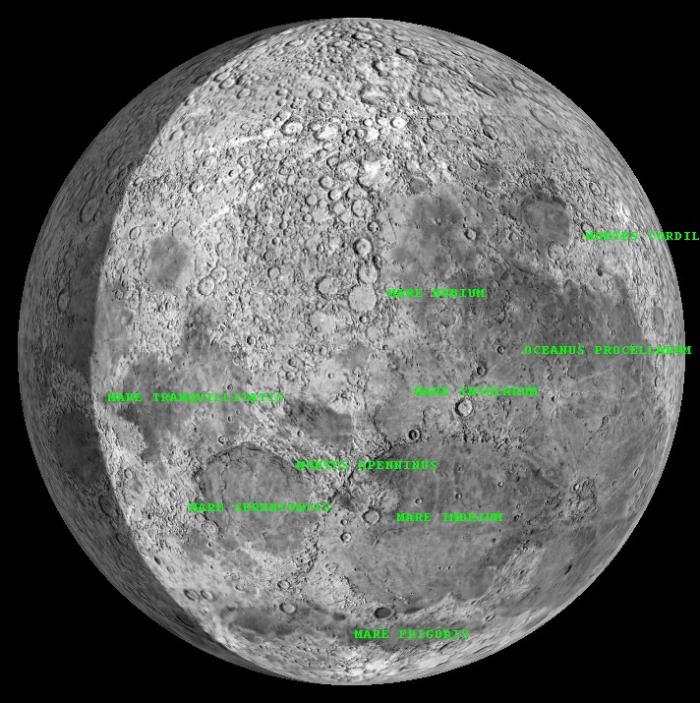
\includegraphics[width=.4\linewidth]{moon.png}
\end{minipage}%
\begin{minipage}{.333\textwidth}
  \centering
  
\includegraphics[width=.8\linewidth]{joshua.png}
\end{minipage}
\begin{minipage}{.333\textwidth}
  \centering
  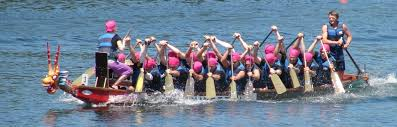
\includegraphics[width=.8\linewidth]{dragonboat.png}
\end{minipage}\\

Joshua has worked full-time for G-Research for 3 years now, and has been actively involved in graduate recruitment since working as a student ambassador following a summer internship. Joshua works as a Machine Learning Analyst, creating financial models to predict investment returns. Many of Joshua�s colleagues have postgraduate degrees, however he recognises that mathematics and computing undergraduate students may have the required skills - in particular, the ability to independently implement theoretical ideas as working code. 

In his spare time, Joshua enjoys dragon boating along the Thames with friends from the office. Joshua also contributes to open source projects, for example a virtual moon atlas. Many students that Joshua meets at career fairs also pursue coding projects in their own time, however Joshua enjoys talking to any bright, enthusiastic and numerate student. Other than a few students that beeline to the G-Research stand, Joshua unfortunately finds it hard to attract attention, as most students flock to famous companies such as Google. When he does manage to attract a student�s attention, he occasionally notices students queueing to talk with him, and then leaving before he gets the chance. 

\subsection{Nicolas}

\begin{minipage}{.333\textwidth}
  \centering
  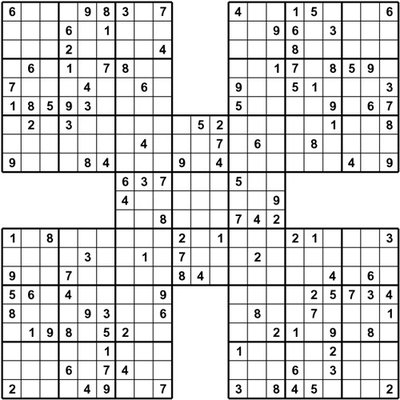
\includegraphics[width=.5\linewidth]{puzzle.png}
\end{minipage}%
\begin{minipage}{.333\textwidth}
  \centering
  
\includegraphics[width=.8\linewidth]{nicolas.png}
\end{minipage}
\begin{minipage}{.333\textwidth}
  \centering
  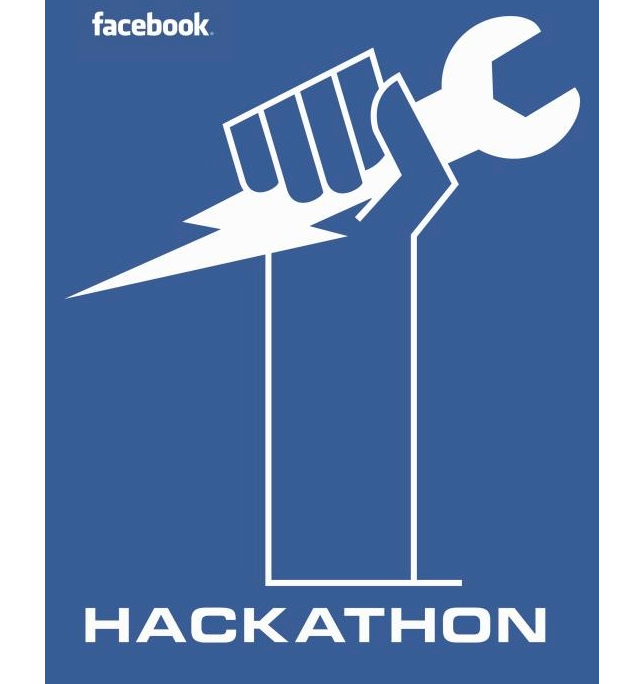
\includegraphics[width=.5\linewidth]{hackathon.png}
\end{minipage}\\

Nicolas is a 3rd year BEng Computing student looking for a graduate role as a developer. He has a lot of programming experience from his degree, so finds it easy to work with new languages and get his head around complicated concepts. He could easily understand a simple API in a few minutes if it is well documented and intuitive. He enjoys puzzles and challenges and takes part in hackathons (such as Facebook Campus hackathons).

He plans to attend the Technology Careers Fair to find companies he would like to work at and apply to. He will attend the stalls of various well known companies, such as Google and Facebook. He is less inclined to talk with smaller companies unless their stand has a specific draw. Nicolas doesn�t want to commit to being at a stand for long time, any activity that takes longer than 10 minutes might dissuade him from visiting a company. 

\section{Value Proposition Canvas TODO TABLE}
We used our personas to create a Value Proposition Canvas that summarizes our understanding of the customer, the product we are producing and the explicit ways it is creating value for both G-Research and the students who will use it. It is clear that the gains/pains and their respective solutions, detailed below, are essentially hypotheses. As we move forwards with user testing it will be interesting to evaluate these proposed gain creators and pain relievers, and pivot development accordingly. We discuss our proposed hallway testing later in this chapter. 

\section{Customer Feedback and Evaluation}
The primary point of contact with our customer, Ed, is our fortnightly sprint review meeting. These take place at the end of each sprint, allowing us to discuss progress made in the previous sprint and any expectations for the next one. To illustrate this let�s examine a previous meeting:
\begin{enumerate}
\item First of all we set up a demo for the latest build of our project. Keeping a clean master branch for our stable code is critical for this, since we wouldn�t want to be running around bug hunting just before Ed arrived.
\item After welcoming Ed to college, we ran through our new features on the demo, highlighting any user stories we successfully implemented. 
\item We explained any scoping decisions we had taken, such as pushing back user stories to the next sprint or pulling them forward. We were not afraid to take full advantage of Ed�s knowledge as a developer, knowing he could understand some of the technical reasons behind the choices we�d made. 
\item  After this we passed the baton over to Ed, allowing him to offer any feedback on the features we�d implemented and discuss if he accepted the user stories as complete or still in need of work. He also discussed how the features fit into his vision of the final product, i.e. if we were making progress or racing off track. This feedback served as a last resort for keeping our goals aligned with our customer, preferably we would know if the feature fit into his vision before we began implementing it.
\item Once the evaluation stage was satisfied we discussed next week�s sprint, in particular the stories he wanted us to work on. We divided these into requirements and stretch goals by estimating the development time required and the importance of the feature. Having this divide between stretch goals and requirements allowed us to balance our time appropriately, making sure we were steadily iterating towards a solid product while also able to add exciting, if not critical, features.
\item Finally we reviewed our progress in regards to the long term picture, considering how far we had made it towards the final product. We considered any features we would likely need to cut or add and planned around this appropriately.
\end{enumerate}

However, limiting contact time to once every two weeks is a dangerous trap to fall into; it leaves little room for us to maneuver around changing customer requirements or our own busy schedules. To help encourage continuous feedback throughout the project, we added Ed to our Trello board. This allows him to keep track of our progress in between face-to-face meetings without adding extra communication overhead on our side. 

As for our communication needs, we can contact Ed in light of developing problems directly via email. One of such issues that arose was what environment we could expect our project to be running in - early in the project we had little knowledge of what technologies G-Research would be willing to support, making design decisions troublesome. It was critical that we got feedback from Ed immediately about what licenses and tools he�d be willing to burden. Leaving such discussions to our next meeting would waste huge amounts of development time in waiting, or scrapping unsuitable work.

On the other hand there are some discussions we can only have with Ed in the room. Some problems simply require throwing ideas back and forth, and the scripting language controlling our cars is a key example. Keeping the design of this approachable enough for a passing student while also offering depth enough for a particularly enthusiastic programmer is a risky balance. Too far one way and the challenge is dull and lifeless, while too far the other way and suddenly you have textbook sized instruction manuals and about one willing participant. The critical importance of this design was not lost on us, so customer feedback was crucial to our development process. Naturally, user testing (as we�ll discuss shortly) also played a strong role in this.

To put it in development terms, continuous feedback from our customer for our evaluation process is similar to the continuous integration approach we used in our design process. Having these short cycles of work followed by review allows us to iterate toward the end game without losing our focus or direction. Maintaining strong communication with our customer is essential to managing our requirements and at the end of the day, making sure we�re implementing something our personas are going to want to use. 

\section{Managing and Prioritising Requirements}
After confirming, or adding, requirements during our customer meeting, the next task is to plan how we will tackle these requirements. As mentioned in the section above, we try to find out during our meetings which features are the highest priority for the customer. This is a good starting point for our internal prioritisation and planning. After a customer meeting we try to meet as a group to prune our product backlog and estimate the size and priorities of our stories for the coming sprint (backlog refinement). You might expect that this is an easy process, as we have found out feature priorities directly from our customer, however this is not the case. With new features it is very difficult to estimate their difficulty. This affects their priority as the amount of time a task takes will affect how achievable it is within our tight timescale. 

A very easy mistake to make would be to jump straight into implementing a new exciting feature that was mentioned in a customer meeting. We avoiding falling into this trap by strictly following the task prioritisation as detailed on our Trello scrum board. For example, before attempting to implement turbo boosts we had to ensure users could edit their AI scripts. Our team may have spent days on implementing turbo boosts, slowly realising that it�s a lot more of a challenge than we initially thought. By the end of the sprint, only half of the new feature may have been built, and the important changes to script editing may not have been made. Script editing is unexciting compared to power-ups, but without it a user�s experience could be made difficult and our own testing would be slowed down.
\subsection{Timeboxed Spikes}
One of the mechanisms that we�ve used to tackle this problem is the use of timeboxed spikes. There have been several occasions in our project where we�ve had difficulty in estimating how long a task will take and thus been apprehensive to begin their implementation. With these tasks it was useful to put some time aside for someone to jump in and see how feasible it is to complete. For example, during our last sprint one of our tasks was to upgrade our racing AI API from a raycast system to a spline-following system. This change was designed to improve the smoothness of the car�s movement and allow for our API to be more easily expanded and simplified. However, we were unsure of how easy this change would be and what benefits it would provide. Therefore, we set aside one afternoon for a member of the team to look into how the change would be made and begin its implementation. We decided that if no decent progress or results had been achieved during this time then we would not continue with the task. Luckily for us, we managed to get one racetrack working with the new system fairly quickly and found out that it did provide many benefits. We then went on to add full support for the system and implemented it on other racetracks.

\subsection{Prototypes}
Another thing that we�ve used to ensure that we�re spending our time on the right things is the use of paper prototypes. When developing new front end systems or features it can be a great time saver to nail down what you want a UI to look like before you begin working on it. Otherwise, a first iteration could be built and then when it�s shown to a stakeholder, the design might turn out to be sub-optimal. The UI may then have to be rebuilt from scratch, in the worst case. Paper prototypes can be used to minimise this wasted time by getting feedback before any time has been spent building it. For example, here is a paper prototype that we used for the script submission page (from the perspective of an anonymous user):

\begin{center}
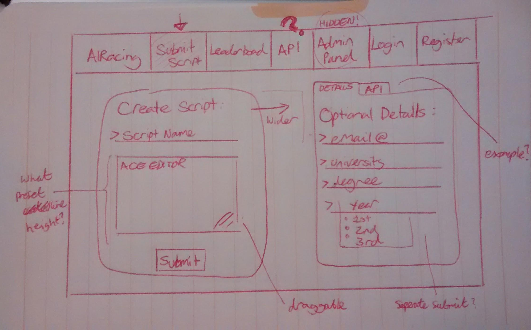
\includegraphics[scale=0.7]{mockup.png}
\end{center}

In our case this was simply used among our team to decide on a design. Which, while not as useful as getting direct customer feedback, allowed us to save time on any later redesigns due to any differences in the imagined look of the site between team members. 

From our experience using UI prototyping software such as Fluid UI, it is rigid and takes only a little less time to create a prototype than drafting up an actual web page. Paper prototypes give the impression that it is a work in process, whereas realistic prototypes can give the impression that too much time and effort has been vested in a UI for it to be changed. We consequently opted for paper prototyping to ensure we received honest feedback from Ed.

\section{Hallway Testing}
Hallway testing is our primary testing method since our target audience, Computing/Maths students, is too small to find reliable statistics through techniques such as the random sampling in A/B testing. Instead, we will setup a mock G-Research careers fair stand with one or two laptops. Our client and a colleague of his will invite students to write AI scripts, and we will assist where appropriate - we will minimise intervention.

We will encourage students to take around 5-10 minutes to write their scripts, as we believe this is representative of how long a student will have at a busy careers fair. Considering only a few laptops will be available, we will provide handouts containing an API reference, short tutorial and space for making notes. Whilst a student waits for a turn on the laptop, this will let them think about the problem and potentially discuss it with other candidates or the recruiters. We will not give the students any help unless required. We will hold regular tournaments during the test and ask students for feedback after submitting their scripts. 

Our primary goal is to promote G-Research, so our project should be exciting for students in order to draw more attention to their stand and consequently generate interest in G-Research. We will evaluate this by observing how much students engage with the game; ideally, there should be some competition to create the fastest script, with students returning to refine their scripts after they are pushed down on the leaderboard. Another key measure will be the time students stay at the stand: we know we need to improve our project if all students spend five minutes on the script and leave immediately afterwards, but we�ve accomplished this goal if students start asking for more time and stay to watch other scripts compete in tournaments.

After the testing, we will discuss how the game generated interest in G-Research with our client and his colleague. From their experience running careers fair stands, it is likely they will have a good idea of whether the software proved valuable as a means of connecting with prospective candidates, or whether it simply functioned as a fun distraction for students. 

An important goal of the project is the usability, as players will have limited means of learning the API given the unconventional setting of a careers fair. It is crucial that the API is easy to use with helpful tutorials and example/starter scripts. We can evaluate the usability by the quality of the scripts, for example, we know the tutorials or the API must be improved if most students submit simple low constant speed scripts or variations of the example scripts. We will ask students to rate the quality of the API, tutorials and example scripts after the test and combine this with our own insights from observing the test to evaluate the usability.

\section{Metrics}
Metrics are an important part of the feedback process. They will allow us to easily understand which parts of the workflow are going right and wrong, in order for us to improve working efficiency. They also allow us to see if our product is working as intended, and what parts need changing - either because they don�t work or as part of general improvement.
\subsection{Workflow Metrics}
Our tasks on Trello currently have story points associated with them, which work as measures of task complexity. We can use this to graph how much work our team can complete in an average iteration, and see if there are any anomalies (which would probably be due to other coursework). We can also use this data to create burndown charts, which allows us to see whether we are going to complete our project on time or whether we will need to adjust our plan accordingly. 

\begin{center}
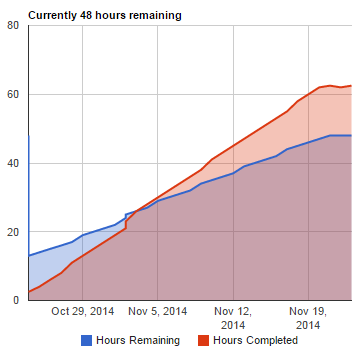
\includegraphics[scale=0.7]{burndown.png}
\end{center}

Creating this graph reveals an alarming trend of an increase in the number of hours remaining. However, this is due to the extra stories we bring into scope after our meetings with our customer go well - so it is not an immediate cause for concern. Reassuringly, our hours completed is fairly linear so we can clearly estimate how productive our team is each week. This makes planning for future weeks simpler as we have a strong idea of how much we can achieve (20 story points).

\subsection{Product Metrics}
We need to be able to evaluate how good a feature is, and quantitatively measure this so we can use it as feedback. There are a few methods for achieving this - for instance, for the website, we can record how long a user spends on a particular page, or how often they visit said page - this represents how popular the feature on the page is. 

It is also useful to determine what exactly users want, and whether we have provided that for them or not. This is usually best implemented as a search function, where we can then see what users searched for against what page they ended up with; however, since this feature isn�t required for our product, we will instead have to use more direct methods such as user surveys, or perhaps a direct feature request button.

On this note, it would also be useful to determine which parts of the product the good candidates look at versus what parts everyone looks at, since this indicates what is interesting to the the type of people G-research want to hire, and means we can focus our development time on improving these parts in particular. For example, a strong candidate may take the time to fully understand the documentation, and would probably be able to improve on existing scripts easily.

We also need to know how interested people are in general - in this case it can be useful to determine how long a user spends against how long they want to spend. For this, we�d need a ratio of the total time spent at the stall and how long the spend writing/racing AI scripts - perhaps they�d want some time to speak to a recruiter but the time spent writing a script was so long they didn�t really have a chance, or wanted to move on to other things.

The racing game is a good opportunity to record various statistics about the user. For instance, when starting the game, we can record which car models and racetracks are played the most, and how many players are commonly in one race. This is useful in deciding what the default settings should be, and also optimising the game for the most common amount of players.


